\setchapterstyle{kao}
\setchapterpreamble[u]{\margintoc}
\chapter{Theory of operation}
\labch{tc-theory-of-operation}

Tesla coils come in a huge variety of sizes, power and modes of operation. From simple spark gap tesla coils, which consist of only a few passive components, to solid state tesla coils, whose only limitations are one's technical skills, every single one amazes anew by combining the world of High Voltage and High Frequency.
\todo[shadow]{Talk about the Nikola Tesla and free energy}

In order to understand the class E topology which this thesis is about, we have to understand the basics first. 

\section{The Tesla Resonator}

A tesla resonator, also called tesla coil, is a resonant transformer consisting of two loosely coupled air-cored windings: the primary and secondary coil. The primary coil, hooked up to the driver circuit on one side and grounded on the other, is usually made out of every few turns of thick wire. It is placed around the bottom of the secondary coil, either shaped like an flat spiral, a concentric cylinder, or at any angle in between. The secondary coil on the other hand has a lot more turns and is a lot higher.

\begin{marginfigure}[*-5]
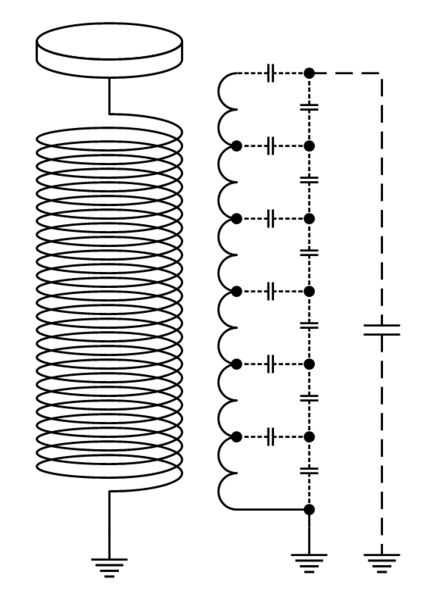
\includegraphics[width=\textwidth]{simon/images/teslaCoilStrayCapacitance.png}
\caption{Stray capacitances of the secondary coil}
\labfig{teslaCoilStrayCapacintance}
\end{marginfigure}

As every real component, a coil has parasitic effects. The one relevant to a tesla coil's operation is the parasitic capacitance. A capacitance is just two different isolated voltage potentials, which is exactly, what we have along every single winding of a coil. This makes clear that every coil is actually an LC oscillator. The lower the inductance and capacitance of the coil, the higher the resonant frequency. This means that in order to lower the frequency to the desired one, many tesla coils have a top load, which, amongst others, acts like as an additional capacity towards ground.

If a high voltage, whose frequency is the resonant frequency of the secondary, is now applied to the primary coil, the LC circuit in the secondary coil starts oscillating and a very high voltage builds up gradually. Depending on the size and power of the tesla coil, this voltage can range from a few thousand to a few million volts. Once the voltage is high enough to ionise the air around the top\sidenote{This usually happens at a designated spark point}, it quickly discharges and the cycle starts over again.

\section{Exciting the resonator}

There are various circuits which can be used for the excitation of the coil. Depending on the desired spark length, size\sidenote{The size of the secondary coil mostly determines its resonant frequency}, sensitivity to external effects, noise level and efficiency, different tesla coil drivers can be used. While Tesla's coils all used a spark gap topology, today we are able to use solid state devices to control the coil instead.

\subsection{The spark gap tesla coil}

\begin{marginfigure}
\missingfigure[figwidth=\textwidwth, figcolor=white]{}
\caption{A simple spark gap tesla coil}
\labfig{teslaCoilStrayCapacintance}
\end{marginfigure}

The simplest of all drivers is the spark gap driver. In the first stage, the 230V mains voltage is transformed to a few kilovolts. Neon sign or microwave transformers are popular choices for this task. The capacitor gets charged up until the voltage is high enough to break through the spark gap. The spark gap then has a very low resistance and allows the current to oscillate between the capacitor and the primary coil. This oscillation frequency is usually in the order of ten to hundred kilohertz and is the same frequency as the resonant frequency of the secondary coil. In every cycle, a little energy is transferred to the secondary via the magnetic coupling of the coils. When the voltage in the secondary gets too high, a breakout occurs. This can happen one or more times within a period of the AC mains voltage. Once all the energy in the primary circuit has been transferred to the secondary or dissipated as heat, the spark gap ''squenches'' allowing the capacitor to charge up again.
